\documentclass[letterpaper]{article}

% AAAI 2027 anonymous submission style
\usepackage[submission]{aaai2027}

% Required packages
\usepackage[hyphens]{url}
\usepackage{graphicx}
\urlstyle{rm}
\def\UrlFont{\rm}
\usepackage{natbib}
\usepackage{caption}
\frenchspacing

% Mathematical formulas
\usepackage{amsmath}
\usepackage{amssymb}

% Professional tables
\usepackage{booktabs}

% Required PDF metadata
\pdfinfo{
/TemplateVersion (2027.1)
}

% Number sections and subsections.
% Subsubsections remain unnumbered.
\setcounter{secnumdepth}{2}

% Paper title
\title{Diffusion-Driven Graph Optimization Framework for Bundle Recommendation}

% Anonymous author information
\author{
Anonymous Submission
}

\affiliations{
}

\begin{document}

\maketitle


\begin{abstract}
Existing bundle recommendation methods typically use multi-view information from user--bundle, user--item, and bundle--item graphs to accurately model users' bundle preferences. However, such multi-view methods still face two key challenges when learning from these graphs: (1) unreliable user--bundle interactions may propagate misleading signals and impair preference learning; (2) the sparsity of user--bundle implicit feedback limits the available supervision. We therefore propose a diffusion-driven graph optimization framework for bundle recommendation (DiGO). First, we aggregate pretrained representations of the bundles in each user's interaction history and condition a diffusion process on the pretrained user representation to model the user's overall bundle preference. We then use this preference representation to score observed user--bundle interactions, retain more reliable user--bundle interactions, and reconstruct the user--bundle graph for subsequent multi-view representation learning. Second, to address the sparsity of user--bundle implicit feedback, we use representations learned from the reconstructed user--bundle graph as anchors and align user--item and bundle--item representations through cross-view contrastive learning before fusing the three views. This allows the auxiliary relations to supplement the limited supervision from user--bundle feedback. Experiments on three public datasets show that our framework outperforms state-of-the-art methods on all evaluation metrics, achieving a maximum relative improvement of 10\% over the strongest baseline.
\end{abstract}


\section{Introduction}

Bundle recommendation aims to identify bundles that match users'
interests from a set of predefined item collections. Existing
methods typically model user--bundle, user--item, and bundle--item
relations jointly and learn complementary user and bundle
representations through graph neural networks, multi-view fusion,
and contrastive
learning~\cite{bgcn,midgn,crosscbr,bundlegt,ma2024multicbr}.
Among these relations, user--item and bundle--item relations
provide auxiliary information, whereas the user--bundle graph
directly carries users' implicit feedback on bundles. Its
structural and supervisory quality therefore affects subsequent
multi-view learning. Despite the progress of existing methods,
multi-view bundle recommendation still faces two key challenges.

\textbf{Challenge 1: Unreliable interactions in the user--bundle
graph.}
User--bundle relations are typically constructed from implicit
feedback and may contain interactions that do not reliably
reflect users' preferences. For example, accidental clicks,
exploratory choices, and interactions caused by short-term
interests or exposure bias may fail to consistently represent
users' actual bundle preferences. Existing graph-based methods
propagate information directly along observed edges, allowing
unreliable interactions to participate in representation updates
and introduce misleading signals. Therefore, identifying more
reliable connections from users' interaction histories and
constructing a high-quality user--bundle graph remain key
challenges.

\begin{figure*}[t]
    \centering
    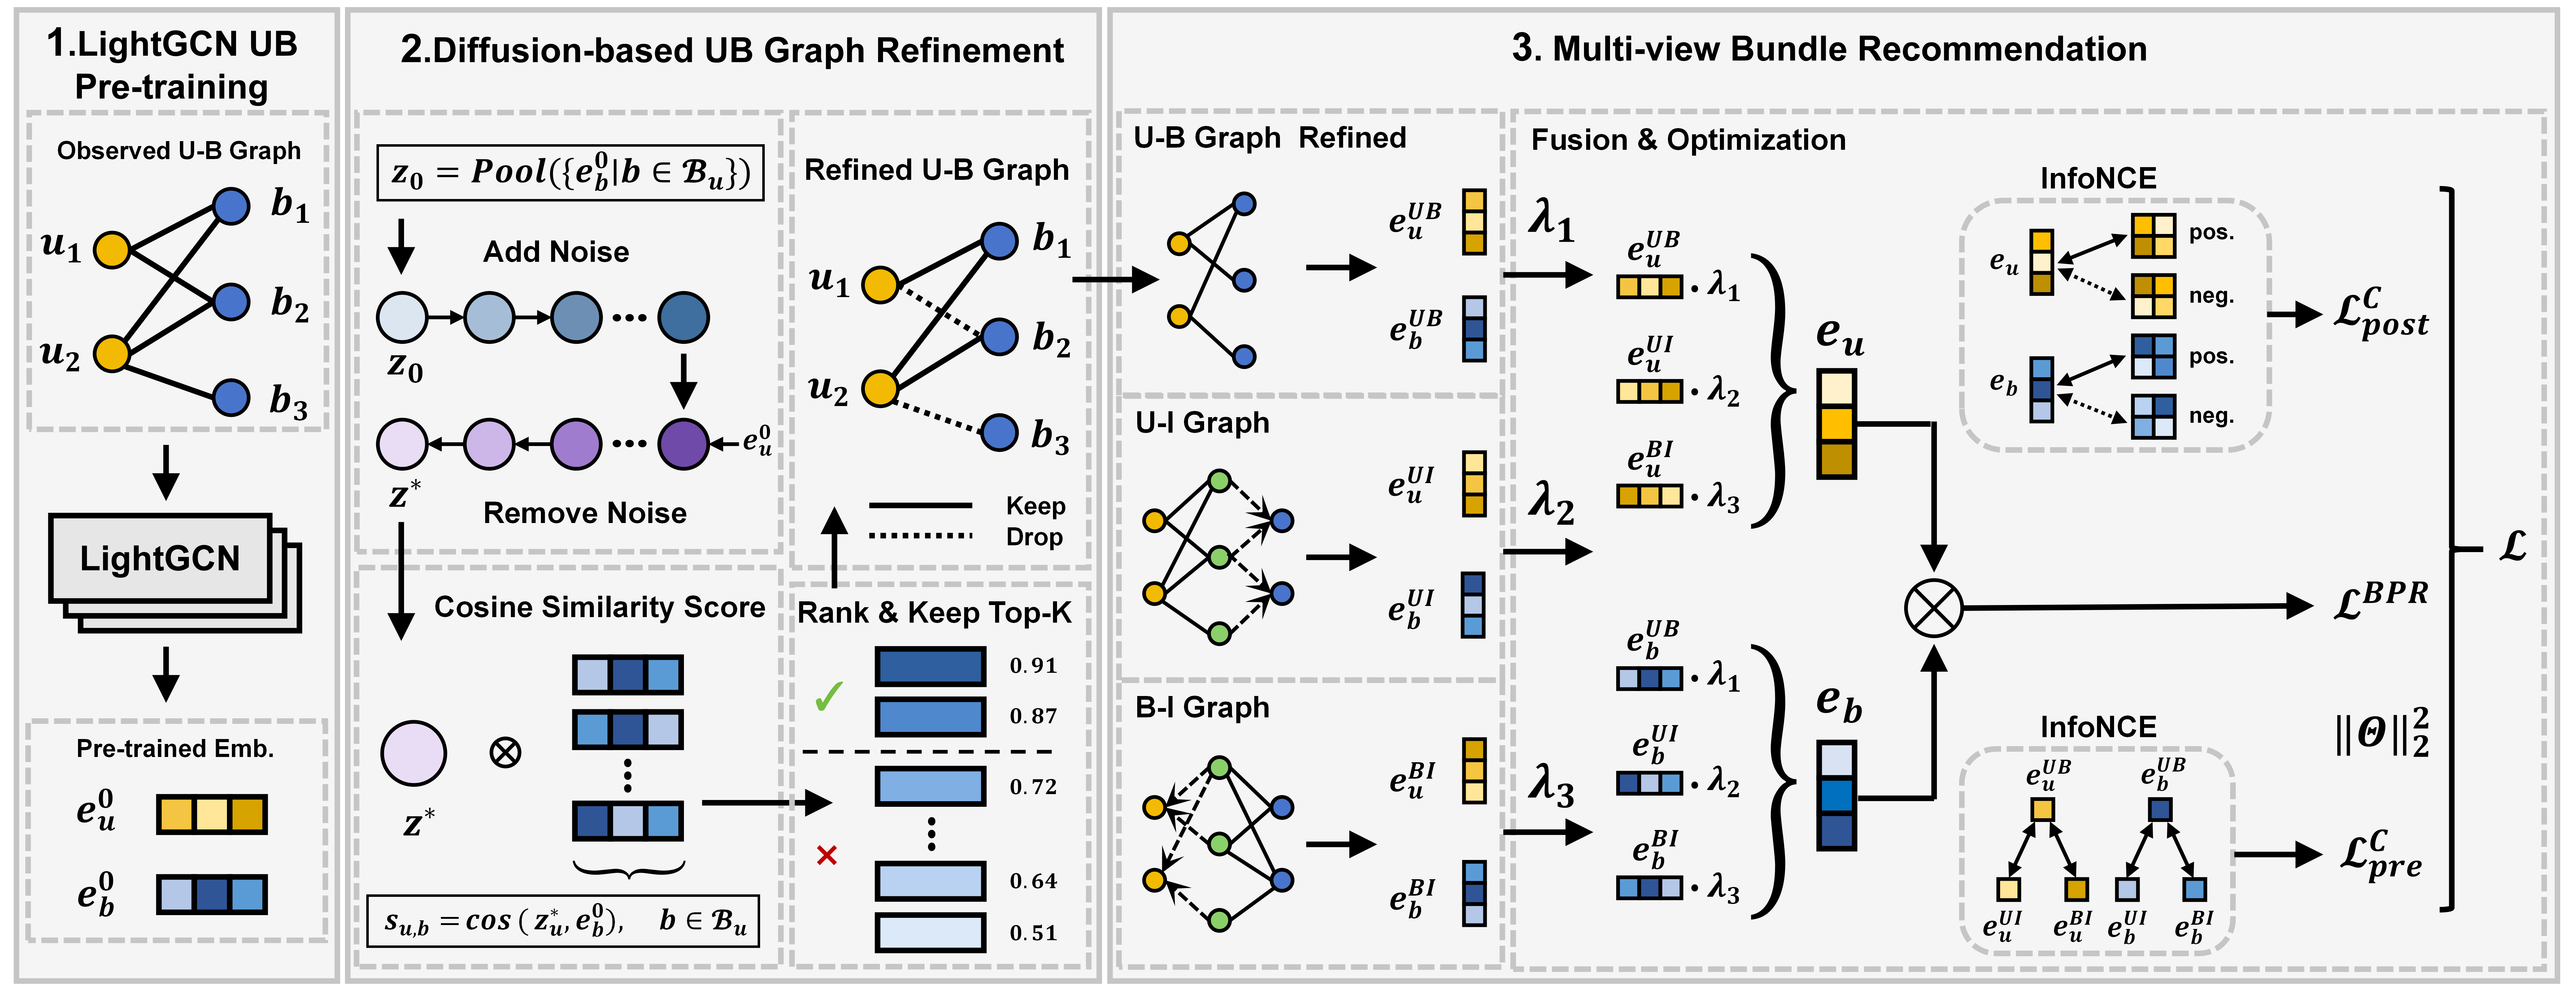
\includegraphics[width=0.98\textwidth]
    {Figures/digo_framework.png}
    \caption{Overall framework of DiGO, comprising (1) user–bundle pretraining, (2) diffusion-driven graph optimization for reconstructing the observed user–bundle graph, and (3) multi-view recommendation using the reconstructed user–bundle view as the anchor for pre-fusion cross-view contrastive learning.}
    \label{fig:framework}
\end{figure*}

\textbf{Challenge 2: Sparse user--bundle implicit feedback.}
User--bundle feedback is substantially sparser than user--item
interactions, providing limited bundle-level supervision.
Although user--item and bundle--item relations offer rich
auxiliary signals, final-stage fusion alone may not fully align
them with user--bundle preference learning. Therefore, effectively
leveraging auxiliary views while preserving consistency with
direct bundle preferences remains challenging.

To address these challenges, we propose DiGO, a diffusion-driven
graph optimization framework for bundle recommendation. DiGO
first aggregates pretrained representations of each user's
historical bundles and conditions a diffusion process on the
pretrained user representation to model the user's overall bundle
preference. The resulting preference representation is then used
to score observed user--bundle interactions, retain more reliable
connections, and reconstruct the graph without introducing new
edges. Finally, DiGO uses representations from the reconstructed
user--bundle graph as anchors to align the user--item and
bundle--item views before fusion, thereby supplementing sparse
supervision. Figure~\ref{fig:framework} illustrates the overall
framework.



The main contributions of this work are summarized as follows:

\begin{itemize}
    \item We propose DiGO, a diffusion-driven graph optimization
    framework that models users' overall bundle preferences
    through conditional diffusion and uses them to re-evaluate
    observed interactions and reconstruct the user--bundle graph.

    \item We use representations learned from the reconstructed
    user--bundle graph as anchors to align the two auxiliary views
    before view fusion, thereby supplementing sparse user--bundle
    supervision.

    \item Experiments on three public datasets show that DiGO
    outperforms existing methods across all evaluation metrics,
    achieving a maximum relative improvement of 10\%. Ablation
    and further analyses also validate the effectiveness of the
    two key designs.
\end{itemize}
\section{Related Work}

\subsection{Bundle Recommendation}

Early bundle recommendation methods primarily relied on
user--bundle interactions and employed collaborative filtering,
matrix factorization, or neural models to learn user and bundle
representations~\cite{earlybundle1,earlybundle2}. Subsequent
graph-based methods further modeled user--bundle, user--item, and
bundle--item relations to capture high-order collaborative
information at both the bundle and item
levels~\cite{bgcn,graphbundle1}.

Recent studies have increasingly focused on multi-view
representation learning and cross-view collaboration. For
example, MIDGN introduces intent disentanglement, CrossCBR
employs cross-view contrastive learning, BundleGT uses graph
Transformers to model structural information, and MultiCBR
learns unified representations through three-view fusion and
contrastive learning~\cite{midgn,crosscbr,bundlegt,ma2024multicbr}.
These methods mainly improve the encoding, fusion, or alignment
of multiple views, while typically using the observed
user--bundle graph directly. In contrast, DiGO re-evaluates
observed user--bundle interactions before multi-view learning and
reconstructs the user--bundle graph accordingly.


\subsection{Diffusion Models for Recommendation}

Diffusion models exhibit strong distribution modeling
capabilities by progressively perturbing data and learning the
corresponding reverse process. In recent years, they have been
applied to collaborative filtering, sequential recommendation,
and knowledge graph recommendation to model user preferences,
recover interaction signals, or enhance recommendation
representations~\cite{diffrec,diffurec,diffkg}.

Diffusion models have also been introduced into bundle
recommendation. RDiffBR addresses dynamic bundle--item relations
by applying residual diffusion to item-level bundle
representations, enabling the model to adapt to changes in bundle
composition~\cite{rdiffbr}. DCBR applies conditional diffusion to
user--bundle interaction data and combines it with multi-view
contrastive learning~\cite{dcbr}. Unlike these methods, DiGO
aggregates the pretrained representations of bundles in each
user's interaction history and conditions the diffusion process
on the pretrained user representation to model the user's overall
bundle preference. The resulting preference representation is
then used to evaluate observed user--bundle interactions and
reconstruct the user--bundle graph for subsequent multi-view
representation learning.



\section{Methodology}

\subsection{Problem Formulation}

Let
$\mathcal U=\{u_1,u_2,\ldots,u_M\}$,
$\mathcal B=\{b_1,b_2,\ldots,b_N\}$, and
$\mathcal I=\{i_1,i_2,\ldots,i_O\}$
denote the sets of users, bundles, and items, respectively, where
$M$, $N$, and $O$ are the corresponding set sizes. We use a
user--bundle interaction matrix
$\mathbf X\in\{0,1\}^{M\times N}$, a user--item interaction
matrix $\mathbf Y\in\{0,1\}^{M\times O}$, and a bundle--item
affiliation matrix $\mathbf Z\in\{0,1\}^{N\times O}$.
Specifically, $x_{ub}=1$ and $y_{ui}=1$ indicate that user $u$
has interacted with bundle $b$ and item $i$, respectively, while
$z_{bi}=1$ indicates that item $i$ belongs to bundle $b$.

Given $\mathbf X$, $\mathbf Y$, and $\mathbf Z$, the goal of
bundle recommendation is to predict the preference score
$y^*_{u,b}$ for each unobserved user--bundle pair.


\subsection{Framework Overview}

As illustrated in Figure~\ref{fig:framework}, DiGO first models
each user's overall bundle preference using pretrained
representations and reconstructs the original user--bundle matrix
$\mathbf X$ as $\widetilde{\mathbf X}$. It then learns user and
bundle representations from three views based on
$\widetilde{\mathbf X}$, $\mathbf Y$, and $\mathbf Z$. Before
fusing the three views, DiGO performs cross-view alignment using
the user--bundle view as the anchor and finally predicts user
preferences from the fused representations.


\subsection{Diffusion-Driven Graph Optimization}

\subsubsection{Preference Representation Construction}

We first pretrain LightGCN~\cite{he2020lightgcn} on the original
user--bundle interactions to obtain pretrained representations
$\bar{\mathbf e}_u$ and $\bar{\mathbf e}_b$ for user $u$ and
bundle $b$, respectively. The pretraining model is optimized with
the BPR objective, and the resulting representations remain fixed
during subsequent graph optimization.

Let
$\mathcal N_u^{UB}
=
\{b\in\mathcal B\mid x_{ub}=1\}$
denote the set of bundles historically interacted with by user
$u$. We construct the historical bundle representation through
mean pooling:

\begin{equation}
\mathbf p_u^0
=
\frac{1}{|\mathcal N_u^{UB}|}
\sum_{b\in\mathcal N_u^{UB}}
\bar{\mathbf e}_b ,
\tag{1}
\end{equation}

where $\mathbf p_u^0$ summarizes the overall characteristics of
the bundles in the user's interaction history and serves as the
modeling target of the subsequent diffusion process.


\subsubsection{Conditional Diffusion}

Given the number of diffusion steps $T$ and a noise schedule
$\{\beta_t\}_{t=1}^{T}$, we define
$\alpha_t=1-\beta_t$ and
$\bar{\alpha}_t=\prod_{s=1}^{t}\alpha_s$.
At timestep $t$, the forward perturbation of $\mathbf p_u^0$ is
defined as

\begin{equation}
\mathbf p_u^t
=
\sqrt{\bar{\alpha}_t}\mathbf p_u^0
+
\sqrt{1-\bar{\alpha}_t}\boldsymbol{\epsilon},
\qquad
\boldsymbol{\epsilon}
\sim
\mathcal N(\mathbf 0,\mathbf I).
\tag{2}
\end{equation}

We use the pretrained user representation
$\bar{\mathbf e}_u$ as a personalized condition and employ a
conditional denoising network to predict the unperturbed bundle
preference representation:

\begin{equation}
\widehat{\mathbf p}_u^0
=
f_\theta
\left(
\mathbf p_u^t,
\bar{\mathbf e}_u,
t
\right),
\tag{3}
\end{equation}

where $f_\theta$ is an MLP-based conditional denoising network
that integrates the perturbed representation, the user condition,
and the timestep embedding.

During training, we uniformly sample $t$ from
$\{1,\ldots,T\}$ and draw Gaussian noise
$\boldsymbol{\epsilon}$ to construct $\mathbf p_u^t$. The
diffusion module is optimized using a representation
reconstruction loss and a historical-set constraint:

\begin{equation}
\begin{aligned}
L_{\mathrm{rec}}^{D}
&=
\mathbb E_{\substack{
u\sim\mathcal U^{+},\,
t\sim\operatorname{Unif}\{1,\ldots,T\},\\
\boldsymbol{\epsilon}\sim\mathcal N(\mathbf 0,\mathbf I)
}}
\left[
\left\|
\widehat{\mathbf p}_u^0-\mathbf p_u^0
\right\|_2^2
\right],
\\
L_{\mathrm{set}}^{D}
&=
\mathbb E_{\substack{
u\sim\mathcal U^{+},\,
t\sim\operatorname{Unif}\{1,\ldots,T\},\\
\boldsymbol{\epsilon}\sim\mathcal N(\mathbf 0,\mathbf I)
}}
\left[
1-
\frac{1}{|\mathcal N_u^{UB}|}
\sum_{b\in\mathcal N_u^{UB}}
\cos
\left(
\widehat{\mathbf p}_u^0,
\bar{\mathbf e}_b
\right)
\right],
\\
L^{D}
&=
L_{\mathrm{rec}}^{D}
+
\eta L_{\mathrm{set}}^{D},
\end{aligned}
\tag{4}
\end{equation}

where
$\mathcal U^{+}
=
\{u\in\mathcal U\mid|\mathcal N_u^{UB}|>0\}$,
$\cos(\cdot,\cdot)$ denotes cosine similarity, and $\eta$
controls the contribution of the historical-set constraint.
$L_{\mathrm{rec}}^{D}$ encourages the prediction to recover the
overall representation of the user's historical bundles, while
$L_{\mathrm{set}}^{D}$ encourages consistency with the actual
bundles in the user's interaction history.


\subsubsection{Interaction Scoring and Graph Reconstruction}

During graph reconstruction, we employ a deterministic iterative
denoising procedure. The historical bundle representation is used
as the initial state, and the conditional denoising network is
repeatedly applied in reverse timestep order:

\begin{equation}
\begin{aligned}
\widetilde{\mathbf p}_u^{T}
&=
\mathbf p_u^0,
\\
\widetilde{\mathbf p}_u^{t-1}
&=
f_\theta
\left(
\widetilde{\mathbf p}_u^{t},
\bar{\mathbf e}_u,
t
\right),
\\
\mathbf p_u^{*}
&=
\widetilde{\mathbf p}_u^{0},
\end{aligned}
\qquad
t=T,T-1,\ldots,1.
\tag{5}
\end{equation}

Here, $\mathbf p_u^{*}$ denotes the resulting overall bundle
preference representation of user $u$.

We then compute preference-matching scores only for the user's
observed interactions and retain at most the top-$\kappa$
bundles:

\begin{equation}
\begin{aligned}
s_{u,b}
&=
\cos
\left(
\mathbf p_u^{*},
\bar{\mathbf e}_b
\right),
\qquad
b\in\mathcal N_u^{UB},
\\
\widetilde{\mathcal N}_u^{UB}
&=
\operatorname{TopK}_{b\in\mathcal N_u^{UB}}
\left(
s_{u,b},
\kappa
\right),
\\
\widetilde{x}_{ub}
&=
\mathbb I
\left[
b\in\widetilde{\mathcal N}_u^{UB}
\right].
\end{aligned}
\tag{6}
\end{equation}

Here, $\kappa$ is the maximum number of interactions retained for
each user, and $\mathbb I[\cdot]$ is the indicator function. All
$\widetilde{x}_{ub}$ form the reconstructed user--bundle matrix
$\widetilde{\mathbf X}$. Since
$\widetilde{\mathcal N}_u^{UB}
\subseteq
\mathcal N_u^{UB}$,
DiGO only re-evaluates and filters observed user--bundle
interactions without introducing unobserved connections.


\subsection{Multi-View Representation Learning}

Based on $\widetilde{\mathbf X}$, $\mathbf Y$, and $\mathbf Z$,
DiGO learns representations from the user--bundle interaction
view, user--item interaction view, and bundle--item affiliation
view. The three views share the initial trainable user, bundle,
and item representations while employing independent propagation
paths.

Let $\operatorname{LG}(\cdot)$ denote a LightGCN encoder with
neighborhood propagation and layer-wise aggregation. The
representation learning process for the three views is written as

\begin{equation}
\begin{aligned}
\left(
\mathbf E_U^{UB},
\mathbf E_B^{UB}
\right)
&=
\operatorname{LG}
\left(
\widetilde{\mathbf X}
\right),
\\
\left(
\mathbf E_U^{UI},
\mathbf E_I^{UI}
\right)
&=
\operatorname{LG}
\left(
\mathbf Y
\right),
\\
\mathbf e_b^{UI}
&=
\frac{1}{|\mathcal N_b^{BI}|}
\sum_{i\in\mathcal N_b^{BI}}
\mathbf e_i^{UI},
\\
\left(
\mathbf E_B^{BI},
\mathbf E_I^{BI}
\right)
&=
\operatorname{LG}
\left(
\mathbf Z
\right),
\\
\mathbf e_u^{BI}
&=
\frac{1}{|\mathcal N_u^{UI}|}
\sum_{i\in\mathcal N_u^{UI}}
\mathbf e_i^{BI}.
\end{aligned}
\tag{7}
\end{equation}

Here, $\mathcal N_b^{BI}$ denotes the set of items contained in
bundle $b$, while $\mathcal N_u^{UI}$ denotes the set of items
interacted with by user $u$. The UB view directly produces the
user representation $\mathbf e_u^{UB}$ and bundle representation
$\mathbf e_b^{UB}$. In the UI view, item representations are
aggregated according to bundle--item affiliations to obtain
$\mathbf e_b^{UI}$. In the BI view, item representations are
aggregated according to user--item interactions to obtain
$\mathbf e_u^{BI}$. This three-view organization follows the
standard multi-view modeling framework for bundle
recommendation~\cite{ma2024multicbr}.

Consequently, user $u$ obtains three view-specific representations
$\{\mathbf e_u^{UB},\mathbf e_u^{UI},\mathbf e_u^{BI}\}$, while
bundle $b$ obtains
$\{\mathbf e_b^{UB},\mathbf e_b^{UI},\mathbf e_b^{BI}\}$.


\subsection{Cross-View Contrastive Learning}

To exploit the two auxiliary views for supplementing sparse
user--bundle supervision, DiGO uses the representations learned
from the reconstructed user--bundle view as anchors and aligns
them with the user--item and bundle--item representations before
fusing the three views.

For an entity set $\mathcal S$, the contrastive loss between an
anchor view $a$ and an auxiliary view $v$ is defined as

\begin{equation}
\begin{aligned}
\ell_{\tau}
\left(
\mathbf E^{a},
\mathbf E^{v};
\mathcal S
\right)
=
-\frac{1}{|\mathcal S|}
\sum_{x\in\mathcal S}
\log
\frac{
\exp
\left(
\cos(\mathbf e_x^{a},\mathbf e_x^{v})/\tau
\right)
}{
\sum_{x'\in\mathcal S}
\exp
\left(
\cos(\mathbf e_x^{a},\mathbf e_{x'}^{v})/\tau
\right)
}.
\end{aligned}
\tag{8}
\end{equation}

Representations of the same entity across the two views form a
positive pair, while representations of the remaining entities
serve as in-batch negatives.

The pre-fusion cross-view contrastive loss is defined as

\begin{equation}
\begin{aligned}
L^{A}
={}&
\ell_{\tau_a}
\left(
\mathbf E_U^{UB},
\mathbf E_U^{UI};
\mathcal S_U
\right)
+
\ell_{\tau_a}
\left(
\mathbf E_U^{UB},
\mathbf E_U^{BI};
\mathcal S_U
\right)
\\
&+
\ell_{\tau_a}
\left(
\mathbf E_B^{UB},
\mathbf E_B^{UI};
\mathcal S_B
\right)
+
\ell_{\tau_a}
\left(
\mathbf E_B^{UB},
\mathbf E_B^{BI};
\mathcal S_B
\right),
\end{aligned}
\tag{9}
\end{equation}

where $\mathcal S_U$ and $\mathcal S_B$ denote the sets of
unique users and positive bundles in the current batch,
respectively, and $\tau_a$ is the temperature parameter. DiGO
only constructs UB--UI and UB--BI alignment on both the user and
bundle sides, without introducing an additional UI--BI
constraint.


\subsection{Prediction and Model Optimization}

The user and bundle representations from the three views are
fused using view coefficients, and their inner product is used
for preference prediction:

\begin{equation}
\begin{aligned}
\mathbf e_u
&=
\lambda_1\mathbf e_u^{UB}
+
\lambda_2\mathbf e_u^{UI}
+
\lambda_3\mathbf e_u^{BI},
\\
\mathbf e_b
&=
\lambda_1\mathbf e_b^{UB}
+
\lambda_2\mathbf e_b^{UI}
+
\lambda_3\mathbf e_b^{BI},
\\
y^*_{u,b}
&=
\mathbf e_u^\top\mathbf e_b,
\qquad
\lambda_1+\lambda_2+\lambda_3=1.
\end{aligned}
\tag{10}
\end{equation}

DiGO also retains post-fusion self-supervised contrastive
learning. Let $\mathbf E'_U,\mathbf E''_U$ and
$\mathbf E'_B,\mathbf E''_B$ denote the user and bundle
representations generated by two independent representation
perturbations, respectively. The post-fusion contrastive loss is

\begin{equation}
L^{C}
=
\frac{1}{2}
\left[
\ell_{\tau_c}
\left(
\mathbf E'_U,
\mathbf E''_U;
\mathcal S_U
\right)
+
\ell_{\tau_c}
\left(
\mathbf E'_B,
\mathbf E''_B;
\mathcal S_B
\right)
\right],
\tag{11}
\end{equation}

where $\tau_c$ is the temperature parameter for post-fusion
contrastive learning.

For each training triplet $(u,b,b')$, where $x_{ub}=1$ and
$x_{ub'}=0$, the recommendation loss and the overall objective
of the multi-view recommendation model are defined as

\begin{equation}
\begin{aligned}
L^{BPR}
&=
\sum_{(u,b,b')}
-\ln
\sigma
\left(
y^*_{u,b}
-
y^*_{u,b'}
\right),
\\
L^{R}
&=
L^{BPR}
+
\beta_1L^{C}
+
\beta_2L^{A}
+
\beta_3
\left\|
\Theta
\right\|_2^2,
\end{aligned}
\tag{12}
\end{equation}

where $\Theta$ denotes the trainable parameters of the multi-view
recommendation model, and $\beta_1$, $\beta_2$, and $\beta_3$
control the contributions of the post-fusion contrastive loss,
the pre-fusion cross-view contrastive loss, and the regularization
term, respectively.

During training, DiGO first optimizes the diffusion module with
$L^D$ and reconstructs $\widetilde{\mathbf X}$. It then uses
$\widetilde{\mathbf X}$, $\mathbf Y$, and $\mathbf Z$ as inputs
and optimizes the multi-view recommendation model with $L^R$.


\subsection{Complexity Analysis}

Let $d$, $K$, and $Q$ denote the embedding dimension, the
number of graph propagation layers, and the number of
recommendation mini-batches per epoch, respectively. Let
$C_f$ denote the cost of one forward pass through the
conditional denoising network. For the fixed-depth MLP used in
DiGO, $C_f=\mathcal O(d^2)$ when its hidden and timestep
embedding dimensions scale with $d$.

Let $\mathcal E_{UB}$, $\mathcal E_{UI}$, and
$\mathcal E_{BI}$ denote the edge sets of the original
user--bundle, user--item, and bundle--item graphs, respectively,
and let $\widetilde{\mathcal E}_{UB}$ denote the edge set of the
reconstructed user--bundle graph. The offline LightGCN
pretraining incurs
$\mathcal O(K|\mathcal E_{UB}|d)$ for graph propagation.
During each DiGO training epoch, diffusion learning costs
$\mathcal O(|\mathcal U^{+}|C_f+|\mathcal E_{UB}|d)$, where
the second term arises from historical bundle aggregation and
the historical-set constraint.

Graph reconstruction further requires
$\mathcal O(T|\mathcal U^{+}|C_f+|\mathcal E_{UB}|d)$ for
iterative denoising and observed-interaction scoring, together
with at most
$\mathcal O(|\mathcal E_{UB}|\log\kappa)$ for top-$\kappa$
selection. The multi-view recommendation component costs
$\mathcal O\!\left(
QKd\left(
|\widetilde{\mathcal E}_{UB}|
+
|\mathcal E_{UI}|
+
|\mathcal E_{BI}|
\right)
\right)$
for graph propagation and
$\mathcal O\!\left(Q(B_U^2+B_B^2)d\right)$
for pre- and post-fusion contrastive learning, where $B_U$ and
$B_B$ are the numbers of unique users and bundles in a
mini-batch, respectively.

Since
$|\widetilde{\mathcal E}_{UB}|
\leq
|\mathcal E_{UB}|$,
DiGO does not increase graph propagation costs through graph
densification and avoids scoring all $M\times N$ user--bundle
pairs. Its parameter space complexity is
$\mathcal O((M+N+O)d+P_f)$, where $P_f$ is the number of
parameters in the conditional denoising network.

\end{document}

